% --------------------------------------------------------------- %
%             3. IOTA PANAUDOJAMUMAS TIEKIMO GRANDINĖSE 
% --------------------------------------------------------------- %

\section{IOTA platformos panaudojimas tiekimo grandinėse} \label{section:application}



% --------------------------------------------------------------- %
%                   3.1. TIEKIMO GRANDINĖS ATVEJIS
% --------------------------------------------------------------- %

\subsection{Tiekimo grandinės atvejis} \label{subsection:sc-example}

Tiekimo grandinės pavyzdinis atvejis buvo kuriamas šio darbo autoriaus, remiantis kelių šaltinių pavyzdinėmis idėjomis~\cite{christopher2016logistics, webber2009building, patrick2017continuous, justin2016customer}. Naudojantis jomis buvo sukurta viena bendra diagrama (žr. priedą~\ref{appendix:1}). 

Diagrama nebuvo siekiama pavaizduoti realaus pasaulio tiekimo grandinės pavyzdžio\footnote{Dėl konfidencialumo priežasčių įmonės nėra linkusios skelbti oficialių savo tiekimo grandinių modelių.}, o labiau siekta sukurti modelį, apimantį kuo daugiau skirtingų tiekimo grandinės fazių ir etapų, kad tai leistų geriau atskleisti IOTA platformos panaudojamumą. Pateiktas modelis galėjo būti dar detalesnis, tačiau tai nebūtinai atspindėtų norimos perteikti esmės.

Šis teikimo grandinės atvejis vaizduoja supaprastintą vaisių tiekimo grandinę nuo ūkininko, įsigyjančio sėklas iki kliento, perkančio vaisius prekybos centre. Tiekimo grandinė išskaidyta į 15 diskrečių etapų, kurių kiekvienas aprašytas atitinkamai.

\medskip \noindent \textbf{1. Ūkininkas superka sėklas iš tiekėjo.} Prieš tai yra sudaromas raštiškas kontraktas tarp sėklų tiekėjo ir ūkininko, kad už tam tikrą kainą ūkininkas gaus tam tikrą kiekį sėklų. Be to, sutartyje gali būti papildomų sąlygų, jei sėklų tiekėjas laiku neturės sėklų arba jų kokybė neatitiks keliamų standartų.

\medskip \noindent \textbf{2. Ūkininkas nurenka pasėtą derlių.} Ūkininkas pasėja vaisių sėklas, sudaro tinkamas sąlygas jų auginimui ir atėjus laikui užaugintus vaisius nurenka ir sandėliuoja. 

\medskip \noindent \textbf{3. Ūkininkas parduoda derlių supirkėjui.} Pardavimas vyksta pagal iš anksto sudarytą kontraktą. Ūkininkas įsipareigoja atėjus konkrečiam terminui parduoti supirkėjui atitinkamą kiekį vaisių, tenkinančių nustatytą kokybės standartą už atitinkamą kainą.

\medskip \noindent \textbf{4. Kurjeris pakrauna vaisius į sunkvežimį.} Supirkėjas samdo kurjerį iš logistikos įmonės, teikiančios transportavimo paslaugas. Supirkėjas gali šiam darbui paskirti ir savo darbuotojus, atsakingus už prekių transportavimą. Pirmuoju atveju būtų sudaromas kontraktas tarp supirkėjo ir logistikos įmonės, įsipareigojančios atgabenti nepažeistas prekes iki nustatyto termino.

\medskip \noindent \textbf{5. Vaisiai transportuojami iki fabriko.}

\medskip \noindent \textbf{6. Vaisiai apdirbami (pagaminami jų išvestiniai produktai) ir sandėliuojami.} Priklausomai nuo vaisių supirkėjo veiklos srities, jis gali vaisius paruošti pardavimui, pvz. apipurkšti cheminiu produktu, suteikiantį blizgumą ar atsparumą, taip pat apdirbti juos supjaustant, panaudojant kaip sudedamąją dalį kituose produktuose ir t.t. Galutiniai produktai sandėliuojami fabriko patalpose, kol atvyks kurjeriai, atsakingi už prekių transportavimą į prekybos centrus. Su prekybos centrais yra pasirašomi kontraktai, nustatantys, kokius produktus už kokią kainą vaisių supirkėjas parduos prekybos centrui.

\medskip \noindent \textbf{7. Apdirbti vaisiai pakraunami į sunkvežimį.} Čia kurjeris gali būti samdomas tuo pačiu principu, kaip ir 4 etape.

\medskip \noindent \textbf{8. Vaisiai transportuojami į jūrų uostą.} Jūrų uostas pagal vidines taisykles perima konteinerį ir paruošia jį pakrovimui į laivą.

\medskip \noindent \textbf{9. Vaisių konteineriai pakraunami į krovininį laivą.}

\medskip \noindent \textbf{10. Krovininis laivas nuplaukia į kitą uostą.}

\medskip \noindent \textbf{11. Vaisių konteineriai iškraunami į sunkvežimius.} Tikėtina, kad kurjeris yra iš tos pačios logistikos kompanijos, kurios sunkvežimis nuvežė konteinerį į pirmąjį jūrų uostą.

\medskip \noindent \textbf{12. Sunkvežimiai išvežioja vaisius į skirtingas šalis.} Transportuojant vaisius yra pasiekiama kitos valstybės siena, kur kurjeris susiduria su muitine.

\medskip \noindent \textbf{13. Muitinėse patikrinami kroviniai.} Priklausomai nuo valstybės, už krovinio įvežimą į šalį gali būti taikomi skirtingi mokesčiai, o kroviniui taikomos skirtingos taisyklės ir standartai. Už atsiskaitymą su muitine yra atsakingas prekybos centras, norintis įsivežti prekes. Atlikus visas būtinas procedūras muitinė išduoda specialų leidimą.

\medskip \noindent \textbf{14. Vaisiai išvežiojami į prekybos centrus.}

\medskip \noindent \textbf{15. Vaisiai parduodami galutiniams pirkėjams.}



% --------------------------------------------------------------- %
%    3.2. TIEKIMO GRANDINĖS ATVEJIS PRITAIKIUS IOTA PLATFORMĄ
% --------------------------------------------------------------- %

\subsection{Tiekimo grandinės atvejis pritaikius IOTA platformą} \label{subsection:application-iota}

Šiame skyriuje autorius pateikia pavyzdinius tiekimo grandinės modelius pritaikius IOTA platformos savybes. Kiekvienas papildytas panaudojimo atvejo etapas arba etapai aprašyti atskirai poskyriuose, pateikiant diagramą su kiekvienu etapo žingsnio detaliu aprašymu.



% --------------------------------------------------------------- %
%                       3.2.1 PIRMAS ETAPAS
% --------------------------------------------------------------- %

\subsubsection{Pirmas etapas} \label{subsection:uc-1}

Pirmojo etapo papildytas modelis, \textit{Ūkininkas superka sėklas iš tiekėjo} (žr.~\ref{img:12} pav.):
\begin{enumerate}
    \item Tarp sėklų pardavėjo ir ūkininko yra sudaromas kontraktas, kad už tam tikrą sumą tam tikru metu ūkininkas galės įsigyti tam tikrą kiekį sėklų. Kontraktas pasirašomas ūkininko ir sėklų tiekėjo, o elektroninė sandorio versija užšifruojama raktu ir gautas šifras patalpinamas į IOTA raizginį. Abi šalys gauna dokumento kopiją ir šifro raktą. Niekas iš IOTA tinklo narių, išskyrus abi kontrakto šalis, negali peržiūrėti kontrakto turinio. Kontrakto šalys gali įrodyti turimos kontrakto kopijos autentiškumą užšifruodami šią kopiją ir patikrindami gauto šifro reikšmę su raizginyje esančiu šifru. Tai leidžia apsisaugoti nuo dokumentų padirbimo arba praradimo juos pametus. 
    \item Sėklų tiekėjas IOTA raizginyje sukuria MAM kanalą, kurį užsiprenumeruoja ūkininkas. Kanalas yra privatus, todėl sėklų tiekėjas prieš tai perduoda specialų raktą ūkininkui, kuris leidžia apsisaugoti, kad duomenų nematytų pašaliniai asmenys. Kanalu perduodami duomenys rašomi į raizginį, o ūkininkas realiu laiku gali stebėti sėklų būseną, pavyzdžiui lokaciją, sandėliavimo sąlygas ir pan.
    \item Sėklų tiekėjas pristato sėklas ūkininkui, o ūkininkas atlieką finansinį pavedimą tiekėjui.
\end{enumerate}

\begin{figure}[H]
    \centering
    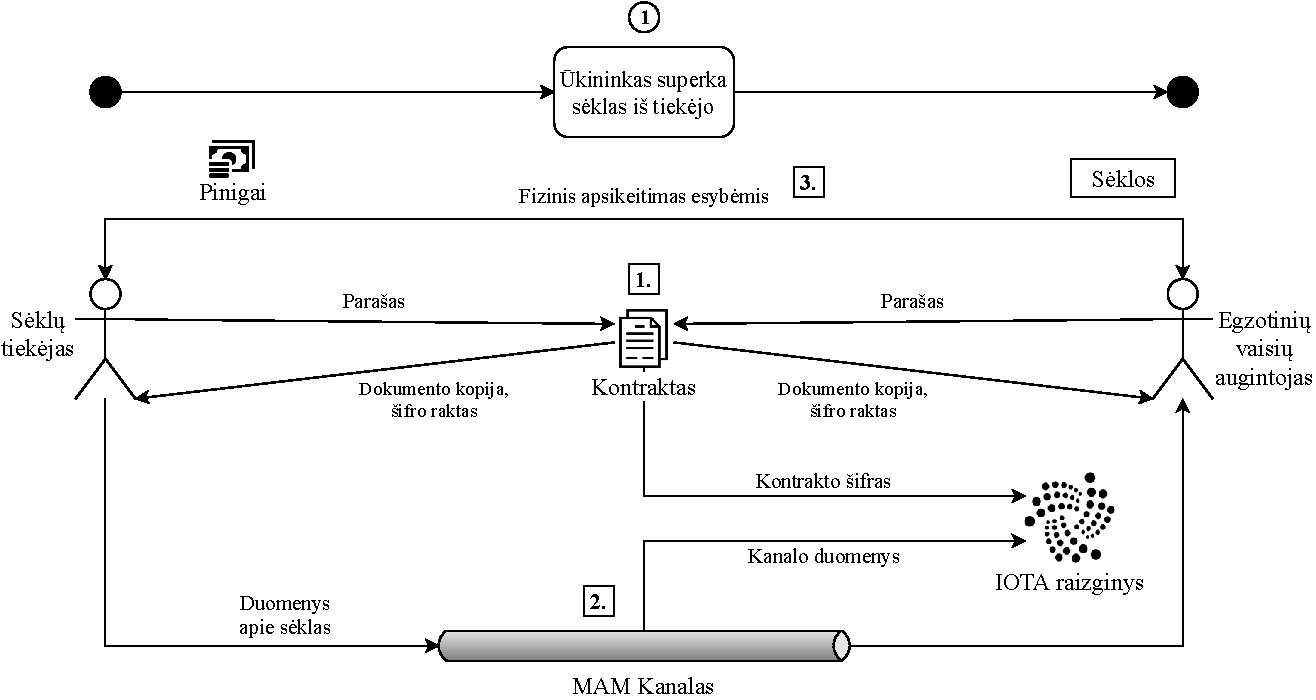
\includegraphics[scale=0.74]{images/iota-usecase-1}
    \caption{1 etapo papildytas modelis}
    \label{img:12}
\end{figure}



% --------------------------------------------------------------- %
%                       3.2.2 ANTRAS ETAPAS
% --------------------------------------------------------------- %

\subsubsection{Antras etapas} \label{subsection:uc-2}

Antrojo etapo papildytas modelis, \textit{Ūkininkas nurenka pasėtą derlių} (žr.~\ref{img:13} pav.):
\begin{enumerate}
    \item Iš pradžių ūkininkas inicijuoja privatų MAM kanalą, kuriuo siųs duomenis potencialiems derliaus supirkėjams. Ūkininkas perduoda kanalo prenumeratos raktą supirkėjui.
    \item Ten, kur yra pasodintos sėklos, pastatomi jutikliai, renkantys duomenis apie aplinką. Šie jutikliai siunčia kanalu duomenis apie vaisių auginimo sąlygas: drėgmę, temperatūrą ir kt. Jutiklius galima būtų sukonfigūruoti, kad kiekvienas atskirai siųstų duomenis į MAM kanalą, arba perduotų duomenis į ūkininko kompiuterį, kuris perimtų duomenų publikavimą.
    \item Esant poreikiui, specialūs IOTA orakulų rolę prisiėmę inspektoriai gali atlikti patikrą, ar jutiklių siunčiami duomenys nėra klastojami ir savo matavimus taip pat patalpinti IOTA raizginyje. Specialūs orakulai galėtų prisidėti ir prie kitų reikalavimų laikymosi patikros. Pavyzdžiui, ar ūkininkas auginimo metu neteršia aplinkos, ar nėra darbinami vaikai ir t.t. Orakulai gali prisidėti ir prie draudimo įmonių veiklos. Esant sausrai ir ūkininkui nepristačius pakankamai derliaus, draudimo kompanijos, gavusios patvirtinimą iš orakulų apie stichinę nelaimę, galėtų padengti ūkininkų nuostolius. Orakulų turėtų dalyvauti kuo daugiau, šitaip užtikrinant, kad daugumos jų parodymai yra objektyvūs ir sutampa. Be orakulų būtų sunku nustatyti, ar jutiklių duomenys, kuriuos teikia ūkininkas, yra nepadirbti. Orakulas duomenis gali perduoti naudojant MAM kanalą.
\end{enumerate}

\begin{figure}[H]
    \centering
    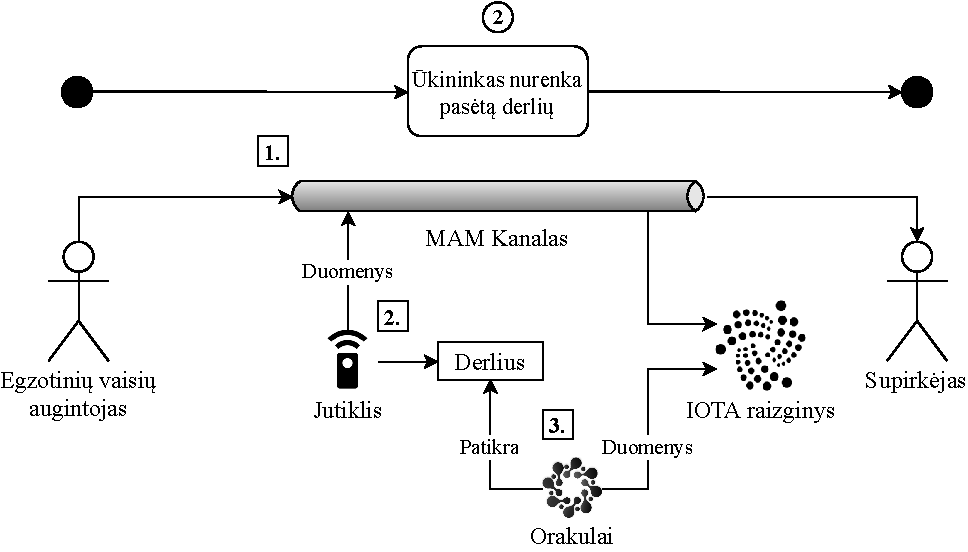
\includegraphics[scale=0.82]{images/iota-usecase-2}
    \caption{2 etapo papildytas modelis}
    \label{img:13}
\end{figure}



% --------------------------------------------------------------- %
%                       3.2.3 TREČIAS ETAPAS
% --------------------------------------------------------------- %

\subsubsection{Trečias etapas} \label{subsection:uc-3}

Trečiojo etapo, \textit{Ūkininkas parduoda derlių supirkėjui} modelio papildymas yra beveik identiškas pirmojo etapo modelio papildymui. Šiuo atveju kontraktas tarp ūkininko ir supirkėjo gali būti sudaromas prieš antrą, o esant poreikiui, ir prieš pirmą etapą tam, kad būtų galima lengviau sekti įsipareigojimų vykdymą.

Svarbu pabrėžti, kad sutarčių ir kontraktų gali būti daugiau nei vienas. Į IOTA tinklą tiekimo grandinės nariai gali įkelti neribotą kiekį bet kokio tipo reikalingų dokumentų.



% --------------------------------------------------------------- %
%                3.2.4 KETVIRTAS IR PENKTAS ETAPAI
% --------------------------------------------------------------- %

\subsubsection{Ketvirtas ir penktas etapai} \label{subsection:uc-4-5}

Ketvirtojo ir penktojo etapų, \textit{Kurjeris pakrauna vaisius į sunkvežimį} ir \textit{Vaisiai transportuojami iki fabriko} bendras papildytas modelis (žr.~\ref{img:14} pav.):
\begin{enumerate}
    \item Pakrovęs vaisius į sunkvežimį kurjeris sukuria MAM kanalą šitaip patvirtinantis perėmęs krovinį ir perimantis atsakomybę už jį\footnote{Paprastai kaskart atlikus transakciją perduodant krovinį, kartu perduodama ir atsakomybė už jį. Tai reiškia, kad krovinį perimanti šalis turi patikrinti krovinio būklę ir su kroviniu susijusius dokumentus, kad būtų galima atrasti pažeidimo priežastį ir kaltininką.}. MAM kanalą prenumeruoja fabrikas\footnote{Šiame tiekimo grandinės pavyzdinio atvejo kontekste fabrikas priklauso supirkėjui.}.
    \item Į MAM kanalą yra perduodami duomenys iš aplinkos jutiklio apie sunkvežimyje esančio krovinio sąlygas ir sunkvežimio lokaciją. Fabrikui (supirkėjui) tai yra naudinga, nes fabrikas gali reaguoti į vaisių atvežimą, pasiruošti jam. Be to, jei vaisiai vėluotų, dingtų bei būtų pristatyti pažeisti arba neatitinkantys kokybės, būtų aišku, kur incidentas įvyko ir kas už tai yra atsakingas.
    \item Vaisiai pristatomi į fabriką, kur yra perduodama atsakomybė už juos.
\end{enumerate}

\begin{figure}[H]
    \centering
    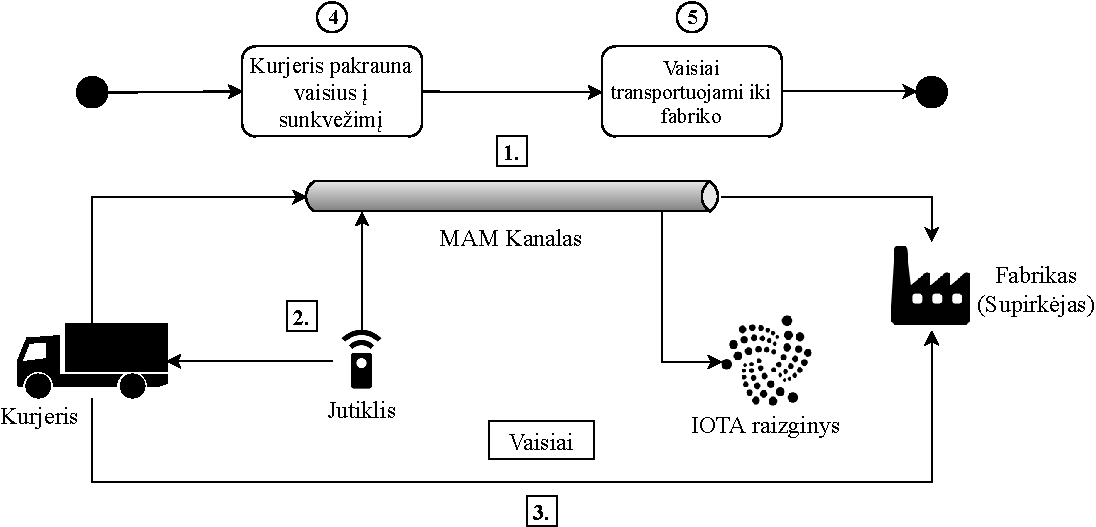
\includegraphics[scale=0.77]{images/iota-usecase-4-5}
    \caption{4 ir 5 etapų papildytas modelis}
    \label{img:14}
\end{figure}



% --------------------------------------------------------------- %
%                       3.2.5 ŠEŠTAS ETAPAS
% --------------------------------------------------------------- %

\subsubsection{Šeštas etapas} \label{subsection:uc-6}

Šeštojo etapo papildytas modelis, \textit{Vaisiai apdirbami (pagaminami jų sub-produktai) ir sandėliuojami} (žr.~\ref{img:15} pav.):
\begin{enumerate}
    \item Kaip ir pirmajame panaudojimo atvejo etape, yra sudaromas kontraktas. Fabrikas (supirkėjas) susitaria su prekybos centru, kad už tam tikrą sumą tam tikru metu bus parduotas tam tikras kiekis perdirbtų arba paruoštų vaisių. Kontraktas pasirašomas abiejų šalių, o elektroninė versija užšifruojama raktu ir gautas šifras patalpinamas į IOTA tinklą \footnote{Kontraktas gali būti sudarytas gerokai anksčiau, pavyzdžiui prieš 1 arba 2 etapą.}. Niekas iš IOTA tinklo narių, išskyrus abi kontrakto šalis, negali peržiūrėti kontrakto turinio. Kontrakto šalys gali įrodyti turimo kontrakto teisiškumą užšifruodami šią kopiją ir patikrindami gauto šifro reikšmę su raizginyje esančiu šifru.
    \item Fabrikas sukuria privatų kanalą, kurį prenumeruoja prekybos centrai\footnote{Jeigu krovinius transportuoja samdomi kurjeriai iš logistikos įmonių, kanalu duomenys gali būti siunčiami ir šiems atstovams, t.y. koks krovinių tipas, kada krovinys paruoštas transportavimui ir t.t.}. Kanalu fabrikas perduoda informaciją apie tai, kokie produktai kuriami, kurioje gamybos stadijoje šie produktai yra esamu laiko momentu, kokiais standartais vadovaujantis apdirbami ir t.t.
    \item Fabrike įtaisyti jutikliai MAM kanalu taip pat perduoda informaciją, pavyzdžiui, gamybos sąlygas skirtinguose etapuose.
    \item Esant poreikiui inspektoriai, kitaip orakulai, gali patikrinti tiek 2, tiek 3 žingsnyje fabriko teikiamą informaciją ir patalpinti į IOTA raizginį prekybos centrams pasitikrinti.
\end{enumerate}

\begin{figure}[H]
    \centering
    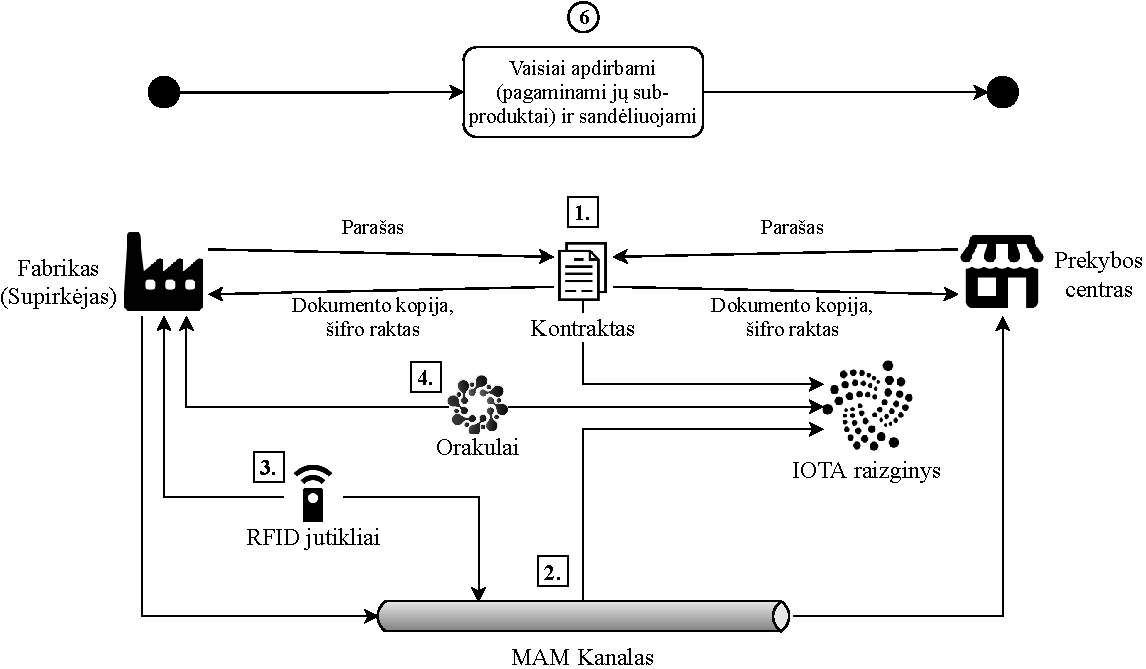
\includegraphics[scale=0.8]{images/iota-usecase-6}
    \caption{6 etapo papildytas modelis}
    \label{img:15}
\end{figure}



% --------------------------------------------------------------- %
%               3.2.6 SEPTINTAS IR AŠTUNTAS ETAPAI
% --------------------------------------------------------------- %

\subsubsection{Septintas ir aštuntas etapai} \label{subsection:uc-7-8}

Septintojo ir Aštuntojo etapų, \textit{Apdirbti vaisiai pakraunami į sunkvežimį} ir \textit{Vaisiai transportuojami į jūrų uostą} bendras papildytas modelis yra beveik identiškas atitinkamai ketvirtojo ir penktojo etapų bendram papildytam modeliui. Kurjeriui sukūrus MAM kanalą, jį prenumeruoja ne tik prekybos centras, bet ir jūrų uostas, kad būtų pasiruošta sunkvežimio atvykimui.



% --------------------------------------------------------------- %
%                3.2.7 DEVINTAS IR DEŠIMTAS ETAPAI
% --------------------------------------------------------------- %

\subsubsection{Devintas ir dešimtas etapai} \label{subsection:uc-9-10}

Devintojo ir dešimtojo etapų, \textit{Vaisių konteineriai pakraunami į krovininį laivą} ir \textit{Krovininis laivas nuplaukia į kitą uostą} bendras papildytas modelis (žr.~\ref{img:16} pav.):
\begin{enumerate}
    \item Vaisių konteineris pakraunamas į krovininį laivą.
    \item Laivas sukuria MAM kanalą, kurį užprenumeruoja kurjeris, laukiantis krovinio jūrų uoste nr. 2. Kanalu perduodama konteinerio su vaisiais laikymo sąlygos, gaunamos iš jutiklių. Laivas išplaukia iš jūrų uosto nr. 1
    \item Laivui plaukiant jūra, dingsta interneto ryšys, tačiau informacijos tiekimas nėra nutraukiamas ir informacijos transakcijos yra toliau atliekamos neprisijungus. 
    \item Po kiek laiko interneto ryšys grįžta ir visos iki tol siųstos žinutės atsiduria IOTA raizginyje, kurias prenumeruotojas gali gauti ir matyti iškart.
    \item Vaisiai transportuojami į jūrų uostą nr. 2.
\end{enumerate}

\begin{figure}[H]
    \centering
    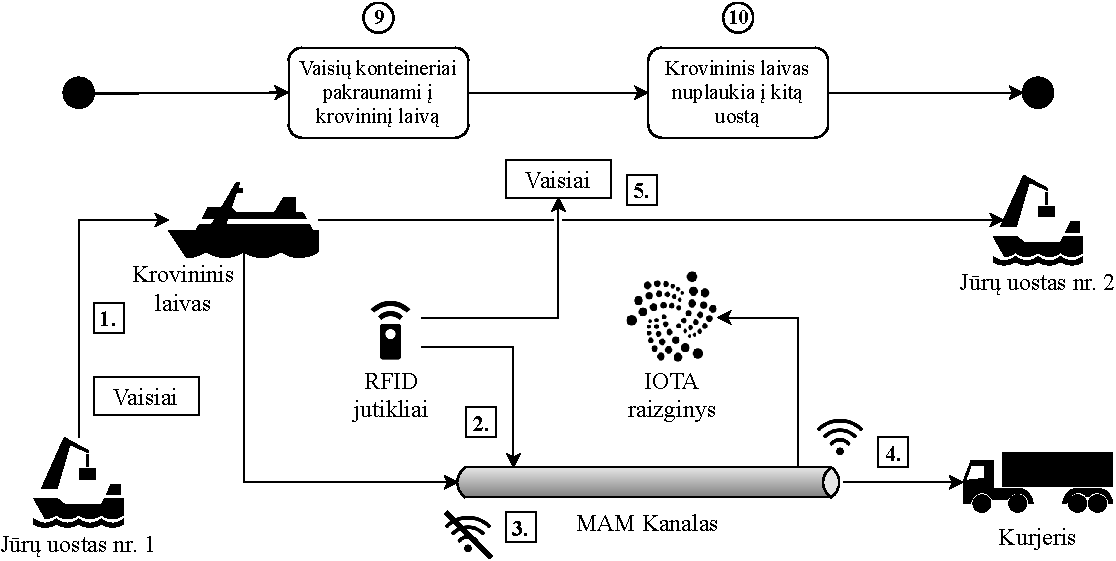
\includegraphics[scale=0.8]{images/iota-usecase-9-10}
    \caption{9 ir 10 etapų papildytas modelis}
    \label{img:16}
\end{figure}



% --------------------------------------------------------------- %
%              3.2.8 VIENUOLIKTAS IR DVYLIKTAS ETAPAI
% --------------------------------------------------------------- %

\subsubsection{Vienuoliktas ir dvyliktas etapai} \label{subsection:uc-11-12}

Vienuoliktojo ir dvyliktojo etapų, \textit{Vaisių konteineriai iškraunami į sunkvežimius} ir \textit{Sunkvežimiai išvežioja vaisius į skirtingas šalis} bendras papildytas modelis (žr.~\ref{img:17} pav.):
\begin{enumerate}
    \item Jūrų uoste nr. 2 iškraunamas konteineris su vaisiais, kurį perima kurjeris.
    \item Kurjeris sukuria MAM kanalą, kurį užprenumeruoja Prekybos centras.
    \item Kurjeris galiausiai pasiekia kitos valstybės muitinę.
\end{enumerate}

\begin{figure}[H]
    \centering
    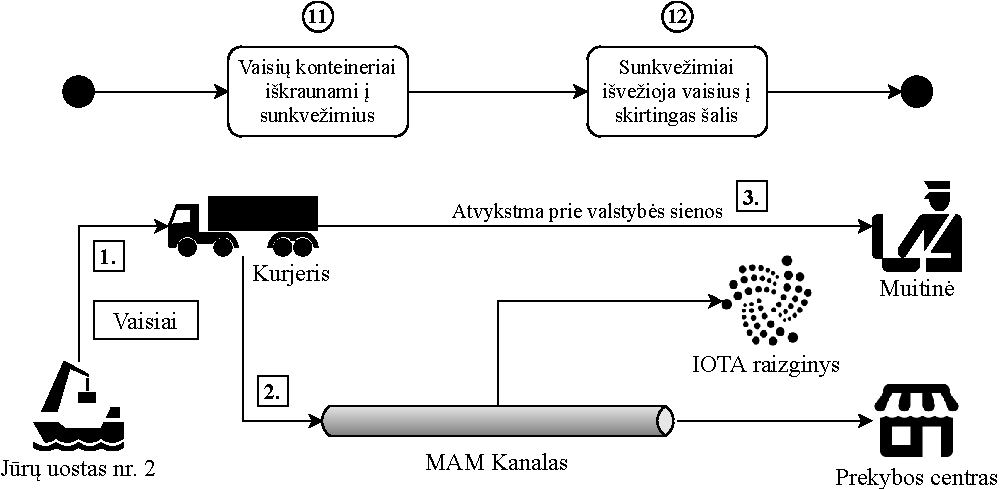
\includegraphics[scale=0.8]{images/iota-usecase-11-12}
    \caption{11 ir 12 etapų papildytas modelis}
    \label{img:17}
\end{figure}



% --------------------------------------------------------------- %
%                       3.2.9 TRYLIKTAS ETAPAS
% --------------------------------------------------------------- %

\subsubsection{Tryliktas etapas} \label{subsection:uc-13}

Tryliktojo etapo papildytas modelis, \textit{Muitinėse patikrinami kroviniai} (žr.~\ref{img:18} pav.):
\begin{enumerate}
    \item Kurjeris perduoda vaisių konteinerį muitinės darbuotojų patikrai.
    \item Muitinės darbuotojai patikrina vaisių kelionės gyvavimo ciklo informaciją IOTA raizginyje. Ši informacija leidžia muitinės darbuotojams lengvai patikrinti svarbią informaciją. Pavyzdžiui, JAV pasienio muitų įstatymas įpareigoja pateikti krovinio pirkėją, pardavėją, gamintoją, kilmės šalį ir kitus duomenis~\cite{customs2018importer}. Visą šią informaciją būtų galima paprastai atsekti ir validuoti IOTA raizginyje, todėl tai galėtų sutaupyti daug laiko. 
    \item Muitinės darbuotojams neradus nieko įtartino, suteikiamas leidimas krovinį įvežti į valstybę. Leidimas taip pat gali būti įrašomas į IOTA raizginį. Vaisius transportuojantis atstovas susimoka muito mokestį (jeigu toks yra taikomas) ir toliau tęsia kelionę.
\end{enumerate}

\begin{figure}[H]
    \centering
    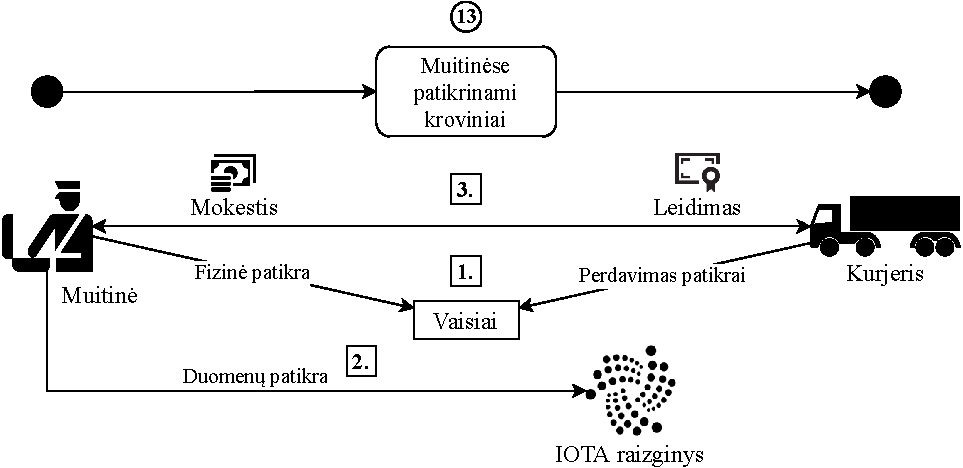
\includegraphics[scale=0.8]{images/iota-usecase-13}
    \caption{13 etapo papildytas modelis}
    \label{img:18}
\end{figure}



% --------------------------------------------------------------- %
%           3.2.10 KETURIOLIKTAS IR PENKIOLIKTAS ETAPAI
% --------------------------------------------------------------- %

\subsubsection{Keturioliktas ir penkioliktas etapai} \label{subsection:uc-14-15}

Keturioliktojo ir penkioliktojo etapų, \textit{Vaisiai išvežiojami į prekybos centrus} ir \textit{Vaisiai parduodami galutiniams pirkėjams} bendras papildytas modelis (žr.~\ref{img:19} pav.):
\begin{enumerate}
    \item Vaisiai transportuojami į prekybos centrą, kuriame šie yra paruošiami pardavimui klientams. Ant vaisių pakuočių prekybos centras pagamina ir užklijuoja specialią informaciją savyje laikantį QR kodo lipduką.
    \item Prekybos centrų klientai nusiperka vaisių pakuotes.
    \item Pirkėjas gali įsitikinti prekybos centro pateikiama informacija, nuskenavęs ant pakuotės esantį QR kodą. Speciali programėlė galėtų leisti peržiūrėti kilmės šalį, vaisių kelionės maršrutą, vaisių auginimo, sandėliavimo ir transportavimo sąlygas, taip pat bet kokią papildomą informaciją, kurią tiekėjai gali atskleisti pirkėjui. Visa ši informacija gaunama iš IOTA raizginyje MAM kanalais bei kitais būdais patalpintos informacijos. Panašiais arba identiškais kodais gali būti žymimi kroviniai visuose tiekimo grandinės etapuose. Pasroviui esantys tiekimo grandinės nariai, prisijungę prie sistemos, galėtų nuskenuoti kodą ir matyti visą jiems aktualią informaciją.
\end{enumerate}

\begin{figure}[H]
    \centering
    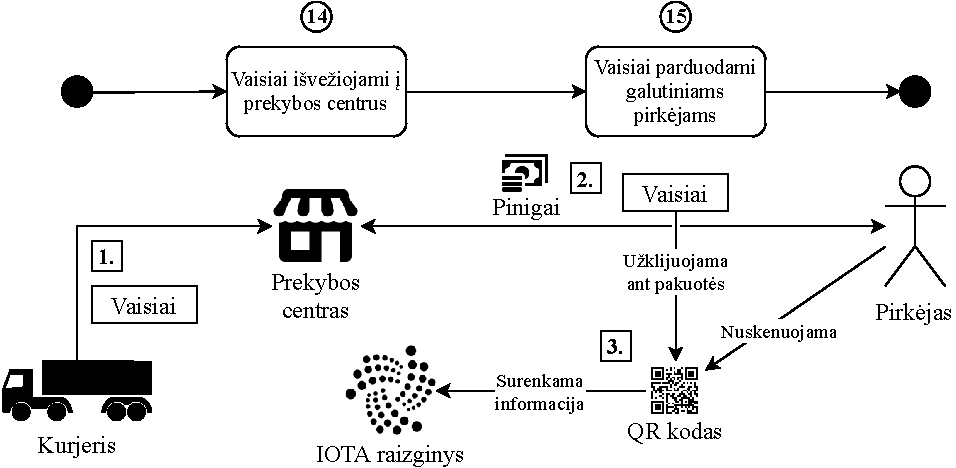
\includegraphics[scale=0.8]{images/iota-usecase-14-15}
    \caption{14 ir 15 etapų papildytas modelis}
    \label{img:19}
\end{figure}



% --------------------------------------------------------------- %
%        3.3 ALTERNATYVŪS IOTA TAIKYMAI TIEKIMO GRANDINĖJE
% --------------------------------------------------------------- %

\subsection{Alternatyvūs IOTA taikymai tiekimo grandinėje} \label{subsection:uc-alt}

3.2. poskyriuose buvo siūlomi IOTA platformos taikymo scenarijai pavyzdinėje tiekimo grandinėje. Tačiau įmanomos įvairios panaudojimo variacijos ir alternatyvos priklausomai nuo situacijos ir poreikio. Šioje dalyje bus nagrinėjamos kelios alternatyvos prieš tai pademonstruotiems panaudojimo atvejo etapų modeliams.

1-12 panaudojimo atvejo etapuose buvo naudojami MAM kanalai. Tačiau šie kanalai buvo sudaromi sukuriant prenumeratos teisę tik pasroviui esančiam tiekimo grandinės dalyviui. Kanalai buvo privatūs, kad informaciją būtų galima siųsti saugiai. Tačiau tiek galutiniai pirkėjai, tiek muitinės, neturėdamos specialaus rakto, gali peržiūrėti tik tą informacinį turinį, kurį pateikia prieš srovę esantis tiekėjas. Vienas iš sprendimo būdų būtų perduoti specialų MAM kanalo prenumeratos raktą visiems pasroviui esantiems tiekimo grandinės dalyviams.

Tačiau tai sukelia papildomų problemų. Skirtingų šalių yra daug: tiesioginiai klientai, netiesioginiai klientai, galutiniai pirkėjai, muitinės ir auditoriai. Visoms šalims reikalinga vis skirtinga informacija. Įmonė nenorėtų, kad konfidenciali informacija, skirta tiesioginiams klientams, pvz. transportavimo tvarkaraščiai arba turimas inventorius, būtų prieinamas galutiniams pirkėjams. Ir atvirkščiai, muitinėms, auditoriams ir galutiniams pirkėjams yra aktuali tik dalis informacijos iš viso srauto.

Naudojant skirtingus MAM kanalus skirstant informaciją tarp tiekimo grandinės šalių ir nustatant skirtingas prieigos teises, galima valdyti informacijos srautus (žr.~\ref{img:20} pav.). Kadangi tiesioginiai klientai keičiasi retai, sukuriamas jam skirtas privatus MAM kanalas. Suvaržytieji kanalai X, Y, ir Z perduoda skirtingus duomenis atitinkamiems prenumeruotojams. Kadangi tiek auditoriai, tiek muitinė, tiek netiesioginiai klientai gali dažnai kisti, yra parenkama suvaržyta kanalų apsauga, leidžianti dinamiškai keisti prenumeruotojus. Viešas kanalas yra skirtas galutiniams pirkėjams, tačiau duomenis gali peržiūrėti bet kas, turintis prieigą prie IOTA raizginio.

\begin{figure}[H]
    \centering
    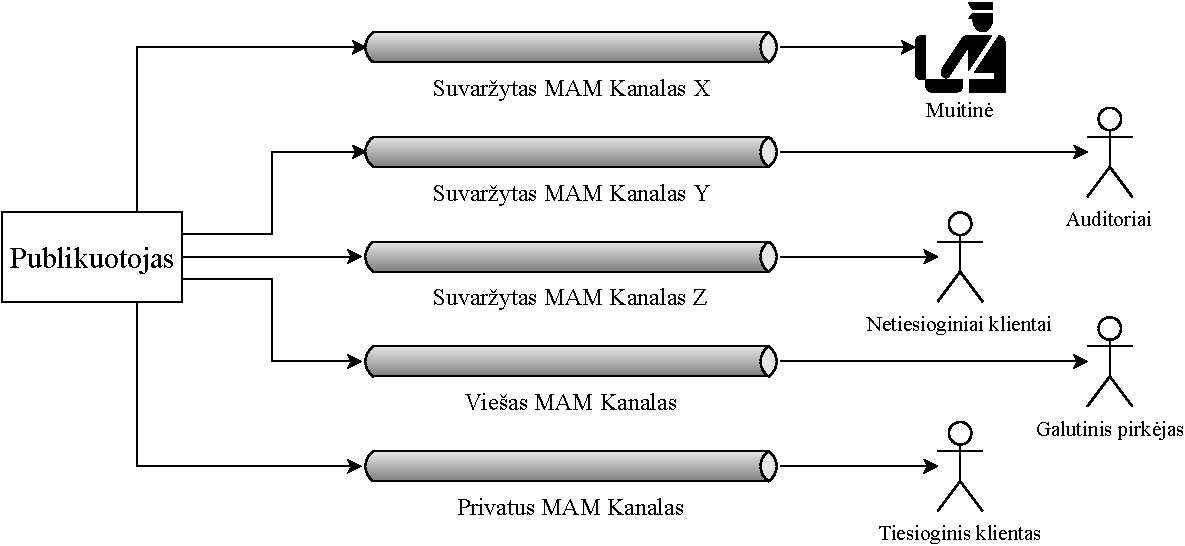
\includegraphics[scale=0.8]{images/mam-channel-flows}
    \caption{Skirtingi MAM kanalų srautai}
    \label{img:20}
\end{figure}

Pavyzdinio panaudojimo atvejo 1, 3, 13-15 etapuose ir bet kuriame kitame etape, kuriame vienas iš žingsnių yra finansinė transakcija, galima naudoti IOTA kaip atsiskaitymo terpę. Tokiam scenarijui pavaizduoti yra tinkamas~\ref{subsection:uc-14-15} poskyryje aprašomas 2 žingsnis. Šiuo atveju galutinis pirkėjas, t.y. prekybos centro klientas perka vaisių pakuotę, už kurią kasoje atsiskaito bankine kortele. Finansine transakcija pasirūpina bankas, o tai, kaip jau buvo minima~\ref{section:dlt} skyriuje, kelia įvairių rizikų.

Tačiau technologijai įsigalėjus klientas galėtų atsiskaityti kriptovaliuta IOTA raizginyje (žr.~\ref{img:21} pav.). Turėdamas savo kriptopiniginę\footnote{Kruptopiniginėje yra laikomos kriptovaliutos. Šiame kontekste kriptopiniginė galėtų būti adresas IOTA raizginyje, kuriame saugomos kriptovaliutos.}, klientas pervestų kriptovaliutą į prekybos centro sąskaitą tiesiogiai ir ši transakcija būtų iškart įrašoma į IOTA raizginį. Tai reiškia, būtų išvengiama tarpininko, šiuo atveju banko. Tokie atsiskaitymai būtų galimi ir didesniais mastais, pavyzdžiui, milijoniniai finansiniai sandoriai tarp verslo šalių. Žinoma, tam reikėtų visuotinio technologijos ir kriptovaliutos pripažinimo ir nusistovėjimo, nes šiuo metu jos kaina labai svyruoja\footnote{Duomenys iš: \href{https://coinmarketcap.com}{https://coinmarketcap.com} [žiūrėta 2019-05-17].}.

\begin{figure}[H]
    \centering
    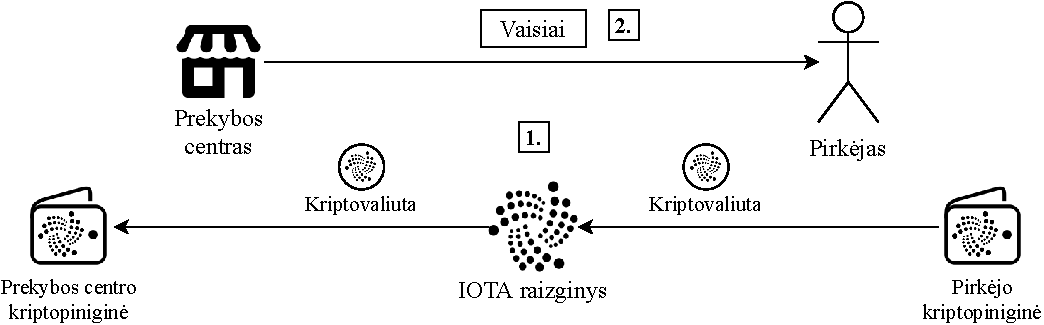
\includegraphics[scale=0.75]{images/tangle-financial-transaction}
    \caption{Finansinė transakcija IOTA raizginyje}
    \label{img:21}
\end{figure}

Pavyzdinio panaudojimo atvejo 2 etape svarbų vaidmenį vaidina orakulai, įrašydami savo duomenis į IOTA raizginį. Tai leidžia patikrinti, ar ūkininko pateikiami duomenys atitinka realybę. Tačiau 2 etapo 3 žingsnį galima praplėsti naudojant orakulus ir išmaniuosius kontraktus (žr.~\ref{img:22} pav.): 
\begin{enumerate}
    \item Geografiniame regione, kuriame ūkininkas augina vaisius, galėtų būti įsikūrę daugybė orakulų, kurie turėtų savo temperatūros matavimo prietaisus. Šiais prietaisais jie pamatuotų temperatūrą arba kitus rodiklius.
    \item Kiekvienas orakulas perduotų savo duomenis išmaniajam kontraktui. Šioje vietoje įmanomas sandorio sudarymas tarp išmaniojo kontrakto savininko ir orakulų. Sandoris įpareigotų orakulus tiekti informaciją išmaniajam kontraktui už tam tikrą kriptovaliutos mokestį.
    \item Išmanusis kontraktas surinktų visų orakulų duomenis ir juos visus perduotų išoriniam skaičiavimų įrenginiui. Atlikus skaičiavimus įrenginys grąžintų gautą skaičiavimų rezultatą išmaniajam kontraktui.
    \item Gautus galutinius skaičiavimus ir kitą informaciją išmanusis kontraktas perduotų MAM kanalu, kurį yra užsiprenumeravęs supirkėjas.
\end{enumerate}

\begin{figure}[H]
    \centering
    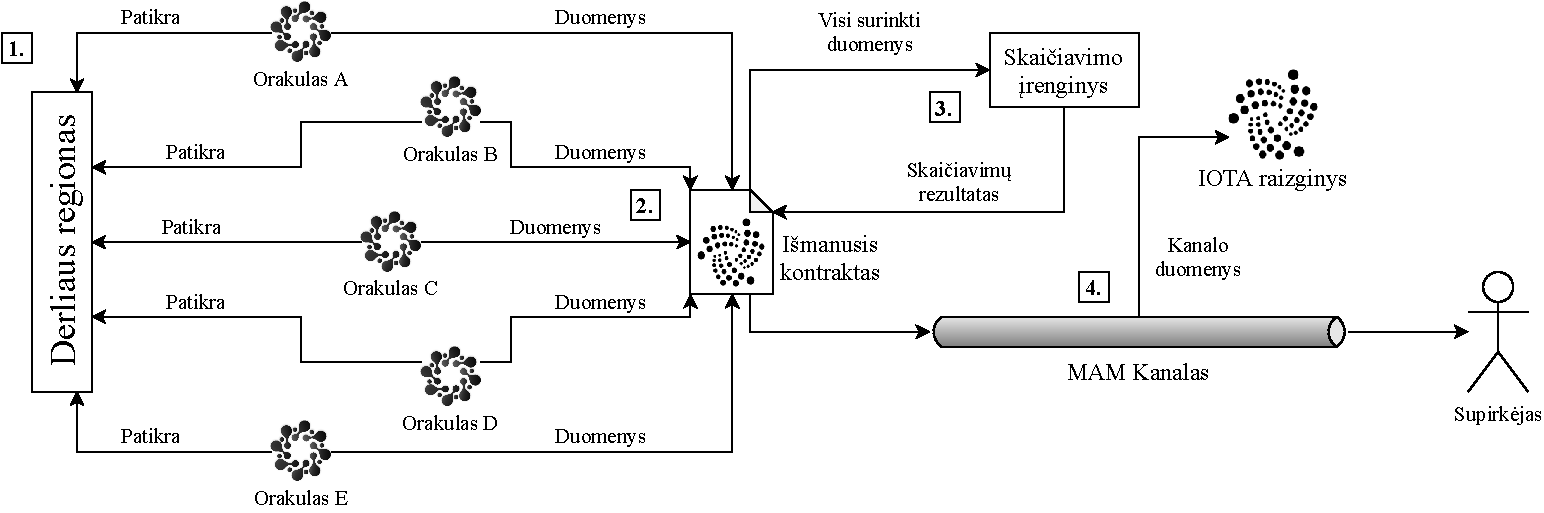
\includegraphics[scale=0.63]{images/tangle-smart-contract}
    \caption{Išmaniojo kontrakto ir orakulų bendradarbiavimas}
    \label{img:22}
\end{figure}



% --------------------------------------------------------------- %
%               3.4 BŪSIMOS SISTEMOS UŽDUOTYS IR VEIKLOS
% --------------------------------------------------------------- %

\subsection{Potencialios sistemos užduotys ir veiklos} \label{subsection:uc-system}

Norint įgyvendinti IT sistemą, įgalinančią IOTA panaudojimą panašioje į tiekimo grandinę, pavaizduotą priede~\ref{appendix:1}, svarbu apsibrėžti sistemoje dalyvaujančias šalis, jų užduotis ir veiklas sistemoje. Remiantis 12-22 paveikslėliuose pavaizduotų siūlomų sprendimų modeliais, buvo surinktos esminės tiekimo grandinės veiklos, kurias galima įgyvendinti potencialioje sistemoje. Taip pat atrinkti visi tiekimo grandinėje esantys dalyviai. Gautas rezultatas pavaizduotas matricoje (žr.~\ref{tab:2} lentelė). 

\begin{table}[h]
\centering
\caption{Skirtingų šalių dalyvavimo tiekimo grandinės procesuose matrica}
\label{tab:2}
\begin{tabular}{|l|l|l|l|l|l|l|l|l|l|l|}
\hline
\textbf{Veikla} & \multicolumn{1}{c|}{\textbf{A}} & \multicolumn{1}{c|}{\textbf{B}} & \textbf{C} & \textbf{D} & \textbf{E} & \textbf{F} & \textbf{G} & \textbf{H} & \textbf{I} & \textbf{J} \\ \hline
Sudaryti sandorį & + & + & + & + & + & + &  & + & + &  \\ \hline
Patikrinti dokumento teisėtumą & + & + & + & + & + & + & + & + & + &  \\ \hline
Sukurti MAM kanalą & + & + & + & + & + & + & + &  & + &  \\ \hline
Prenumeruoti MAM kanalą &  & + & + & + & + & + & + & + & + & + \\ \hline
Siųsti kriptovaliutą &  & + & + &  & + &  &  &  & + & + \\ \hline
Gauti kriptovaliutą & + & + & + & + & + & + &  & + & + & + \\ \hline
Perduoti duomenis išmaniajam kontraktui &  &  &  &  &  & + &  &  &  &  \\ \hline
Generuoti QR kodą &  & + & + & + & + &  & + & + &  &  \\ \hline
Nuskaityti QR kodą &  &  & + & + & + &  & + & + &  & + \\ \hline
\end{tabular}
\end{table}

Lentelė reikalauja specialaus paaiškinimo. Kiekvienas stulpelio antraštės simbolis A-J reiškia vis skirtingą tiekimo grandinėje dalyvaujančią rolę. A – sėklų tiekėjas, B – ūkininkas, C – vaisių supirkėjas, D – kurjeris, E – prekybos centras, F – orakulas, G – muitininkas, H – jūrų uostas, I – išmaniojo kontrakto savininkas, J – galutinis pirkėjas. Langeliai su „+“ simboliu reiškia, kad atitinkama tiekimo grandinės šalis dalyvauja tam tikrame procese.

Autorius pastebi, kad potenciali sistema gali turėti daugybę kitų funkcionalumų, tokių kaip registracija, prisijungimas, istorijos peržiūra ir t.t. Tačiau šiame darbe nagrinėjamos pagrindinės bazinės sistemos veiklos, tiesiogiai susijusios su IOTA taikymo tiekimo grandinėje pavyzdžiais. 

Dar vienas svarbus reikalavimas, kurį turi įgyvendinti sistema – tai nuolatinė prieiga prie IOTA raizginio. Tai yra būtina tam, kad sistemos ir raizginio duomenys visada būtų sinchronizuoti ir būtų remiamasi naujausia raizginio informacija. Tam užtikrinti reikalingas interneto ryšys. Nors, kaip jau minėta~\ref{subsection:dag-offline} ir~\ref{subsection:uc-9-10} poskyriuose, tam tikrais atvejais sistema būtų galima naudotis ir neturint interneto prieigos.

Kiekviena ~\ref{tab:2} lentelėje pažymėta veikla turi būti prieinama atitinkamoms šalims per sistemos naudotojo sąsają naudotojui prisijungus. Tai reiškia, kad turi būti sukuriamos skirtingos sistemos būsenos priklausomai nuo to, koks naudotojas yra prisijungęs. 

Tam, kad skaitytojui būtų paprasčiau įvertinti, ką ir kaip potenciali sistema turėtų atlikti, darbo autorius siūlo supaprastintus sistemos veiklų scenarijus, kuriems buvo nubraižytos panaudos atvejų ir veiklų UML diagramos. Visos diagramos buvo parengtos remiantis matricos duomenimis (žr.~\ref{tab:2} lentelė) naudojant \textit{draw.io} naršyklės įrankį. 

Priede~\ref{appendix:2} ir priede~\ref{appendix:3} pavaizduotos sistemos užduočių diagramos, parodančios sistemos rolių (angl. \textit{Actors}) galimas užduotis. Prieduose nr. 4-8 pavaizduotos veiklų diagramos, parodančios kaip ir kokiais scenarijais įvairios rolės ir sistema bendrauja tarpusavyje.